%%%%%%%%%%%%%%%%%%%%%%% file template.tex %%%%%%%%%%%%%%%%%%%%%%%%%
%
% This is a general template file for the LaTeX package SVJour3
% for Springer journals.          Springer Heidelberg 2010/09/16
%
% Copy it to a new file with a new name and use it as the basis
% for your article. Delete % signs as needed.
%
% This template includes a few options for different layouts and
% content for various journals. Please consult a previous issue of
% your journal as needed.
%
%%%%%%%%%%%%%%%%%%%%%%%%%%%%%%%%%%%%%%%%%%%%%%%%%%%%%%%%%%%%%%%%%%%
%
% First comes an example EPS file -- just ignore it and
% proceed on the \documentclass line
% your LaTeX will extract the file if required
%\begin{filecontents*}{example.eps}
%%!PS-Adobe-3.0 EPSF-3.0
%%%BoundingBox: 19 19 221 221
%%%CreationDate: Mon Sep 29 1997
%%%Creator: programmed by hand (JK)
%%%EndComments
%gsave
%newpath
%  20 20 moveto
%  20 220 lineto
%  220 220 lineto
%  220 20 lineto
%closepath
%2 setlinewidth
%gsave
%  .4 setgray fill
%grestore
%stroke
%grestore
%\end{filecontents*}
%
\RequirePackage{fix-cm}
%
%\documentclass{svjour3}                     % onecolumn (standard format)
%\documentclass[smallcondensed]{svjour3}     % onecolumn (ditto)
%\documentclass[smallextended]{svjour3}       % onecolumn (second format)
\documentclass[twocolumn]{svjour3}          % twocolumn
%
\smartqed  % flush right qed marks, e.g. at end of proof
%
\usepackage{graphicx}
%
% \usepackage{mathptmx}      % use Times fonts if available on your TeX system
%
% insert here the call for the packages your document requires
%\usepackage{latexsym}
% etc.
%
% please place your own definitions here and don't use \def but
% \newcommand{}{}
%
% Insert the name of "your journal" with
 \journalname{Autonomous Robots}
%
\begin{document}

\title{Working title%\thanks{Grants or other notes
%about the article that should go on the front page should be
%placed here. General acknowledgments should be placed at the end of the article.}
}
\subtitle{Humans helping robots helping humans}

%\titlerunning{Short form of title}        % if too long for running head

\author{Deepak E. Gopinath$^*$      \and
        Brenna D. Argall %etc.
}

%\authorrunning{Short form of author list} % if too long for running head

\institute{ Deepak Gopinath \at
            Department of Mechanical Engineering\\
            Northwestern University, Evanston, IL\\
              Tel.: +123-45-678910\\
              Fax: +123-45-678910\\
              \email{deepakgopinath@u.northwestern.edu}           %  \\
%             \emph{Present address:} of F. Author  %  if needed
           \and
           Brenna Argall \at
}

\date{Received: date / Accepted: date}
% The correct dates will be entered by the editor


\maketitle

\begin{abstract}
Assistive human cyber-physical systems have the potential to transform the lives of millions of people afflicted with severe motor impairments as a result of spinal cord or brain injuries. The effectiveness and usefulness of assistive systems, however, is closely related to their ability to infer the user's needs and intentions and is often a limiting factor for providing appropriate assistance \textit{quickly, confidently and accurately}. The contributions of this paper are two-fold: firstly, we leverage the notion of \textit{inverse legibility} and propose a goal disambiguation algorithm which enhances the intent inference and assistive capabilities of a shared-control assistive robotic arm. Secondly, we introduce a novel intent inference algorithm that works in conjunction with the disambiguation scheme, inspired by dynamic field theory in which the time evolution of the probability distribution over goals is specified as a dynamical system. We also present a experimental study to evaluate the efficacy of the disambiguation system. This study was performed with ten subjects. Results show that upon operating the robot in the control mode picked by the disambiguation algorithm, the progress towards the goal significantly became faster as a result of accurate and confident robot assistance and the number and rate of mode switches performed by the user decreased as well. 
\keywords{Shared Autonomy \and Intent Inference \and Intent Disambiguation \and Assistive Robotics}
% \PACS{PACS code1 \and PACS code2 \and more}
% \subclass{MSC code1 \and MSC code2 \and more}
\end{abstract}

\section{Introduction}\label{intro}
%Assistive Robotics and what it can do

Assistive and rehabilitation machines---such as assitive robotic arms, exoskeletons and powered wheelchairs---have the potential to transform the lives of millions of people with severe motor impairments. These devices can promote independence, boost self-esteem and help to extend the mobility and manipulation capabilities of such individuals, thereby revolutionizing the way motor-impaired people interact with society. With the rapid technological strides in the domain of assistive robotics, the devices have become more capable and complex---to the extent that control of these devices becomes a greater challenge. 

The control of an assistive device is typically facilitated via a control interface. The greater the motor impairment of the user, the more limited are the interfaces available for them to use. These interfaces (for example, Sip-N-Puff and switch-based head arrays) are low dimensional, discrete interfaces that can operate only in subsets of the entire control space. 
The dimensionality mismatch between the control interfaces and the controllable degrees-of-freedom of the assistive robot necessitates the partitioning of the entire control space into smaller subsets called \textit{control modes}. In order to achieve full control of the robot, the user switches between the control modes and this is referred to as \textit{mode switching} or \textit{modal control}. More importantly, as the control interface becomes more limited and low-dimensional, the greater number of control modes there are. 




Complexity of device and dimensionality mismatch. Control modes etc. Switching between modes is hard, gets in way of task execution. Therefore shared autonomy. 

What is shared autonomy. Different types of Shared autonomy. Common factor in all is that for successful assistance nad robot behavior intent infernece is important 

Understanding intent is critical. Why? Shared intention in human-human teams. Human-robot teams. Different types of paradigms exist for the same. 

Intent inference is harder in assistive domain, due to sparsity of signals. Could supplement it using other tyoes of sensor data, but makes it less practical and possibly affect user acceptance due to the cumbersome nature. 

But we have human-in-th-loop. If the robot can elicit more intent expressive actions from the user, the inference problem becomes easier for the robot. Therefore the intent disambiguation system. 


\section{Related Work}\label{sec:1}
Text with citations \cite{McGeer01041990}
\section{Mathematical Algorithm and Implementation}\label{MAI}
%\subsection{Subsection title}\label{sec:2}
%as required. Don't forget to give each section
%and subsection a unique label (see Sect.~\ref{sec:1}).
\subsection{Intent Disambiguation}
\subsection{Intent Inference and Shared Control}\label{IISC}
\section{Experimental Design - Study Methods}
\section{Results}
\section{Discussion}
\section{Conclusion}


%% For one-column wide figures use
%\begin{figure}
%% Use the relevant command to insert your figure file.
%% For example, with the graphicx package use
%  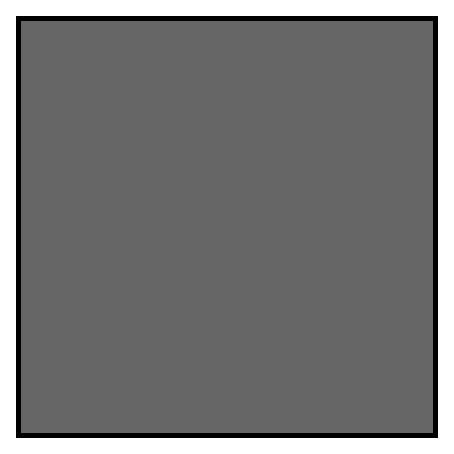
\includegraphics{example.eps}
%% figure caption is below the figure
%\caption{Figure1}
%\label{fig:1}       % Give a unique label
%\end{figure}
%%
%% For two-column wide figures use
%\begin{figure*}
%% Use the relevant command to insert your figure file.
%% For example, with the graphicx package use
%  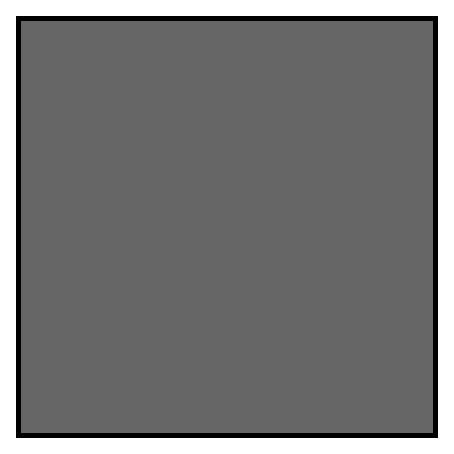
\includegraphics[width=0.75\textwidth]{example.eps}
%% figure caption is below the figure
%\caption{Figure2}
%\label{fig:2}       % Give a unique label
%\end{figure*}
%%
%% For tables use
%\begin{table}[h!]
%% table caption is above the table
%\caption{Please write your table caption here}
%\label{tab:1}       % Give a unique label
%% For LaTeX tables use
%\begin{tabular}{lll}
%\hline\noalign{\smallskip}
%first & second & third  \\
%\noalign{\smallskip}\hline\noalign{\smallskip}
%number & number & number \\
%number & number & number \\
%\noalign{\smallskip}\hline
%\end{tabular}
%\end{table}


\begin{acknowledgements}
If you'd like to thank anyone, place your comments here
and remove the percent signs.
\end{acknowledgements}

% BibTeX users please use one of
\bibliographystyle{spbasic}      % basic style, author-year citations
%\bibliographystyle{spmpsci}      % mathematics and physical sciences
%\bibliographystyle{spphys}       % APS-like style for physics
\bibliography{references}   % name your BibTeX data base

% Non-BibTeX users please use
%\begin{thebibliography}{}
%%
%% and use \bibitem to create references. Consult the Instructions
%% for authors for reference list style.
%%
%\bibitem{RefJ}
%% Format for Journal Reference
%Author, Article title, Journal, Volume, page numbers (year)
%% Format for books
%\bibitem{RefB}
%Author, Book title, page numbers. Publisher, place (year)
%% etc
%\end{thebibliography}

\end{document}
% end of file template.tex

